	\begin{align}
	\vec{C} = \frac{\vec{A+B}}{2} 
	\implies 	\vec{A} = 2\vec{C}-\vec{B} 
	 = \myvec{3\\-10\\}	
	\end{align}       
	The radius is then obtained as
\begin{align}
	\norm{\vec{B}-\vec{C}} = 5\sqrt{2}
\end{align}
	See 
\figref{fig:chapters/10/7/2/7Fig}.
\begin{figure}[H]
\begin{center}	
	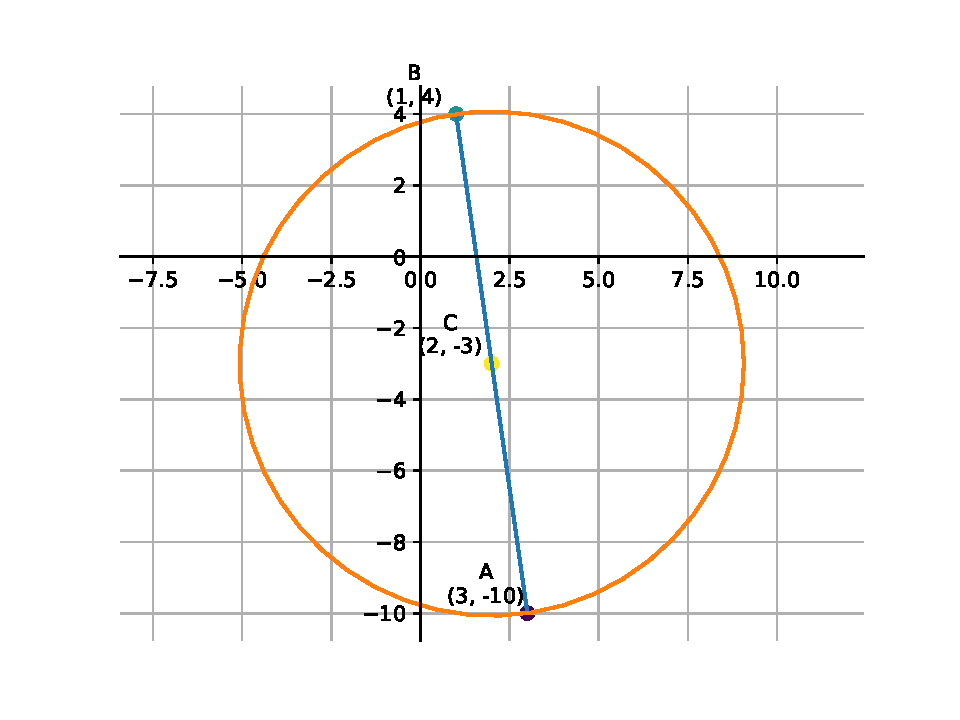
\includegraphics[width=0.75\columnwidth]{chapters/10/7/2/7/figs/fig.pdf}
\end{center}
\caption{}
\label{fig:chapters/10/7/2/7Fig}
\end{figure}
	
